% ~~~ [ MC-Semantics ] ~~~~~~~~~~~~~~~~~~~~~~~~~~~~~~~~~~~~~~~~~~~~~~~~~~~~~~~~~

\subsubsection{MC-Semantics}
\label{sec:rel_work_mc-semantics}

The MC-Semantics project may be used to decompile native code into LLVM IR. MC-Semantic conceptually consists of two components which separate concerns related to the disassembly stage (see section \ref{sec:lit_review_disassembly}) from those of the intermediate code generation stage. Firstly, the control flow recovery component analyses binary files (e.g. ELF, PE files) and disassembles their machine instructions (e.g. x86 assembly) to produce a serialized CFG (in the Google Protocol Buffer format) which stores the basic blocks of each function and the native instructions contained within. Secondly, the instruction translation component converts the native instructions of the serialized CFG into semantically equivalent LLVM IR.

The clear separation between the two decompilation stages in MC-Semantics has enabled two independent implementations of the control flow recovery component in two different programming languages (i.e. C++ and Python), thus validating the language-agnostic aspects of its design. The C++ component is called \texttt{bin\_descend} and it implements a recursive descent disassembler which translates the native code into serialized CFGs. As described in section \ref{sec:lit_review_disassembly}, implementing a disassembler which correctly separates code from data is made difficult by a range of problems; e.g. indirect branches, intermixed code and data in executable segments, callbacks. Interactive disassemblers (such as IDA) solve these issues, by relying on human problem solving skills to resolve ambiguities and inform the disassembler. The second implementation of the control flow recovery component is an IDAPython script which produces serialized CFGs from IDA Pro.

The interaction between the components of the MC-Semantics project is illustrated in figure \ref{fig:mcsema_overview}.

\begin{figure}[htbp]
	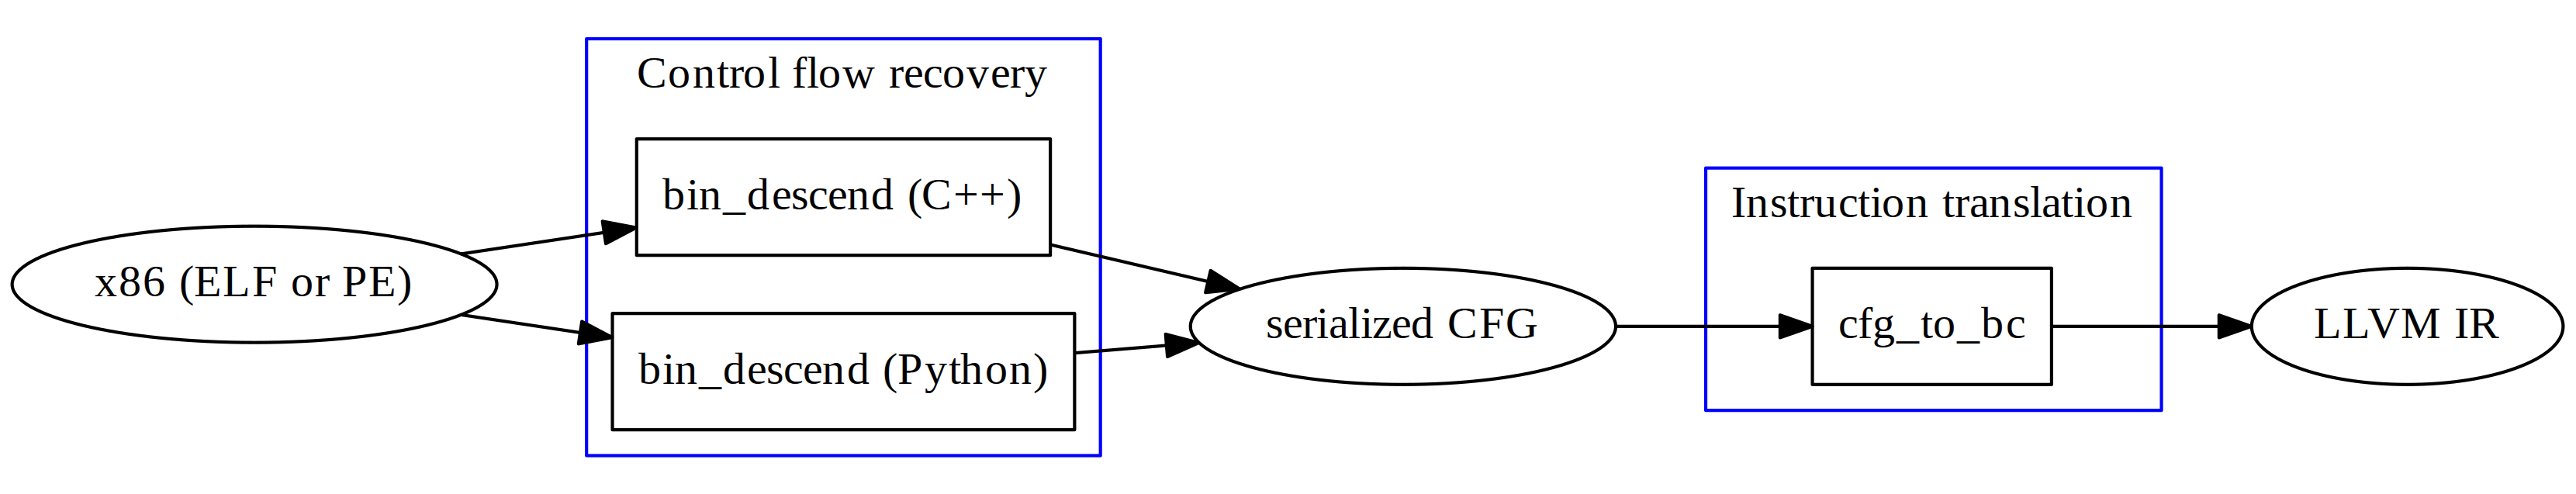
\includegraphics[width=\textwidth]{inc/3_rel_work/mcsema_overview.png}
	\caption{foo}
	\label{fig:mcsema_overview}
\end{figure}

Dagger and MC-Semantics uses a structure to keep track of all registers and passes a pointer to this structure as an argument to each function. Reads from and writes to registers are made using loads and stores.

% TODO: Evaluate and highlight key differences between Dagger, Fracture and McSema.
% Dagger and Fracture rely on TableGen for instruction semantics, McSema does not.

% TODO: Research; https://github.com/trailofbits/mcsema

% TODO: Re-watch the youtube talk again.

% bin_descend and IDA python script of MC-Semantics -> Google Protocol Buffer -> cfg_to_bc -> LLVM IR

An demonstration foo is presented in appendix \ref{app:mc-semantics_example}.

foo \cite{mcsema}

% TODO: Verify supported formats.
* MC-Sema support:

PE (x86)
COFF (x86)
ELF (x86)

% TODO: Mention how semantic analysis could improve the output.
